\chapter{Introduction}

\section{Background}

During disasters such as earthquakes, Urban Search And Rescue (USAR) robots are used to detect victims in hazardous environments where first responders would otherwise be put at risk. Advanced USAR robots can explore and map the environment while overcoming obstacles, and deliver supplies to victims who cannot be immediately evacuated. USAR robots were first used in the aftermath of the September 11 attacks on the World Trade Centre, where they had limited success as they would frequently get stuck or damaged. Since then, designs for USAR robots with many different locomotion methods have been considered and compared in competitions such as the RoboCup Rescue Robot League and the DARPA Robotics Challenge. At present, USAR robots are typically only successful at surveillance; due to the extreme conditions in disaster zones and the urgency of rescue operations, first responders will rarely consider using USAR robots.\\

\begin{wrapfigure}{r}{0.35\textwidth} %this figure will be at the right
	\centering
	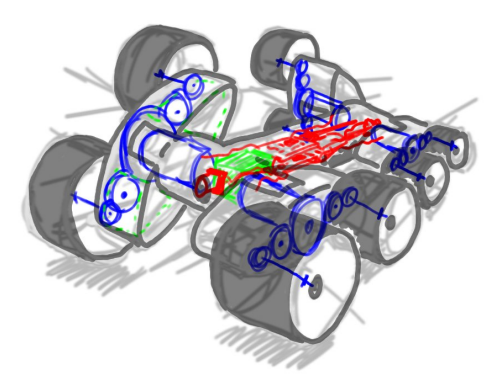
\includegraphics[width=0.35\textwidth]{Wilson-sketch}
	\caption{Systems layout of Wilson's LIM device \citep{Wilson-2013}}
	\label{Wilson sketch}
\end{wrapfigure}

\noindent Another problem limiting the use of USAR robots is cost; USAR robots are prohibitively expensive so rescue organisations use them sparingly. There is a need for low-cost, expendable USAR robots. In 2013, Matthew Wilson proposed an automatically-shape-shifting platform that uses a Load Intuitive Module (LIM) in the place of regular wheels, shown in Figure \ref{Wilson sketch} \citep{Wilson-2013}. The LIM system uses two outer "minor wheels" placed on a central hub that can be rotated as a "major wheel". The minor wheels are geared to the central hub such that they drive the vehicle, however if they experience high resistance, for example from hitting an obstacle, the torque will cause the major wheel to rotate instead, flipping one of the minor wheels over the obstacle to automatically climb it. This is a strong concept for an inexpensive stair-climbing robot as it only uses a single motor for both normal driving and climbing obstacles.\\



\noindent "LIMed" robot platforms (platforms using LIMs for locomotion) were built individually by four final year students at UCT \citep{Wilson-2013},  \citep{Haskel-2017}, \citep{Buchanan-2018}, and \citep{Powrie-2019}. One of these robots is shown in Figure \ref{Powrie robot}. These platforms show some success in climbing a single step, albeit inconsistently. Powrie noted that a mathematical model that accurately describes the kinematics of the system could be developed to optimise the design of LIMed robots. This project is a continuation of these students' work.


\begin{figure}[h]
	\centering
	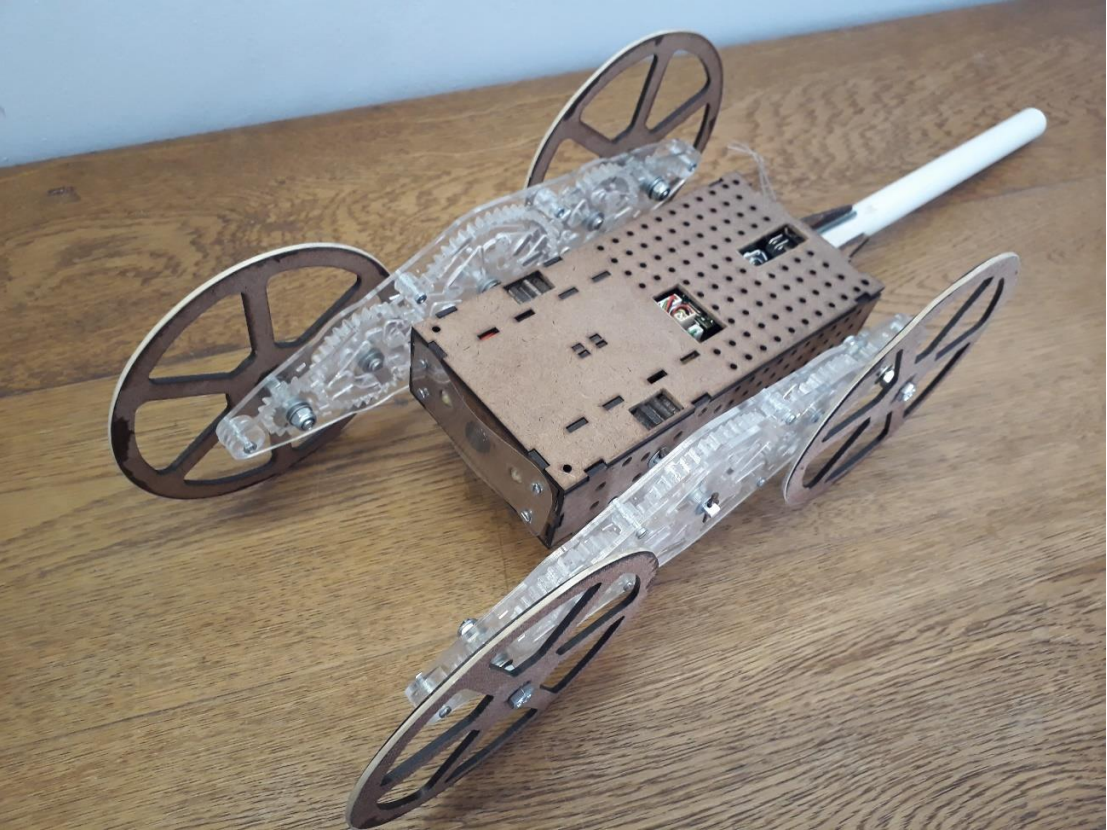
\includegraphics[width=0.4\textwidth]{Powrie-device}
	\caption{Powrie's "Di-Wheel" robot \citep{Powrie-2019}}
	\label{Powrie robot}
\end{figure}

\section{Objectives}
The aim of this project is to create a model that can be used to inform future USAR designs.
The following objectives were identified to meet this aim:
\begin{enumerate}
	\item Create a model to describe the kinematics of a LIM.
	\item Build a prototype USAR device which uses LIMs to climb stairs.
	\item Validate the model using the prototype.
\end{enumerate}
This project does not intend to create a fully functioning USAR robot, but rather a prototype of the platform that a USAR robot may use.
\section{Motivation}

Many designs for USAR locomotion exist, however highly capable devices are prohibitively expensive. There remains a need for USAR devices that are both affordable and effective, and LIMed USAR robots could fill that role in the near future. Designers will be able to use the model produced in this report to design and optimise LIMed USAR robots. These robots use fewer actuators so could be cheaper than existing USAR robots. Lowering the cost of USAR robots is a priority as it makes them more accessible to rescue organisations.